\section{Nonlinear Transformation}
\noindent
{\color{LightRubineRed} \rule{\linewidth}{1mm} }
%%%%%%%%%%%%%%
\begin{align*}
x \in \mathcal{X} \overset{\Phi}{\rightarrow} \ z \in \mathcal{Z}
\end{align*}
perceptrons in $Z$-space = quadratic hypotheses in $X$-space \par
%%%%%%%%%%%%%%
Linear/simpler model first. \par
\begin{center}
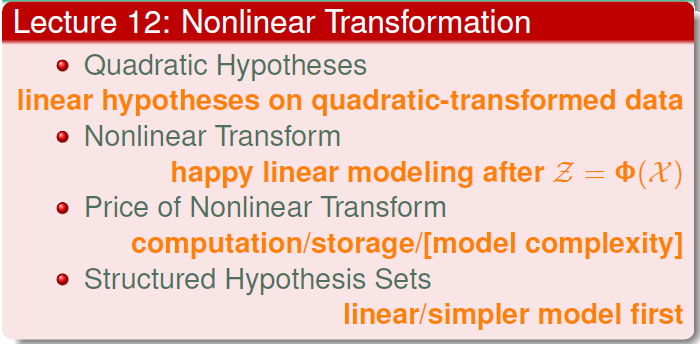
\includegraphics[width=10cm, height=5cm]{lecture12_sum}\\
\end{center}
\noindent
{\color{RubineRed} \rule{\linewidth}{1mm} }